\documentclass[letterpaper,11pt]{article}
\usepackage{standalone}
\usepackage[spanish]{babel}
\usepackage[utf8]{inputenc}
\usepackage[binary-units]{siunitx}
\usepackage{amsthm}% http://ctan.org/pkg/amsthm
\usepackage[left=2.5cm, top=2.5cm, right=2.5cm, bottom=3cm]{geometry}
\usepackage{lastpage}
\usepackage{fancyhdr}
\usepackage{multicol}
\usepackage{hyperref}
\usepackage{color}
\usepackage[binary-units]{siunitx}
\usepackage[american,siunitx]{circuitikz}
\usepackage{placeins}
\usepackage[shortlabels]{enumitem}
\usepackage{tcolorbox}

\newcommand{\unidad}[1]{\,\si{#1}}
\fancyfoot[C]{\thepage\ de \pageref{LastPage}}

\begin{document}
\thispagestyle{empty}
% MATERIA
\newcommand{\materia}{\uppercase{Control i}}
% MAESTRO
\newcommand{\maestro}{\uppercase{Gerardo Marx Chavez Campos}}

% TIPO DOCUMENTO
\newcommand{\tipoDoc}{\uppercase{REPORTE DE LABORATORIO}} %TAREA, REPORTE DE LABORATORIO,
% NOMBRE DE DOCUMENTO
\newcommand{\nombreDoc}{\uppercase{Práctica 2}} 
% NUMERO DE DOCUMENTO (SI ES NECESARIO)
\newcommand{\docNum}{}
% SUBNOMBRE DOCUMENTO
\newcommand{\subNombreDoc}{\uppercase{Búsqueda de polos y ceros por inspección}}

% ALUMNOS 
\newcommand{\alumnos}{\uppercase{GABRIEL AGUILAR LEMUS \\ josé pablo barragán franco}}
% FECHA DE ENTREGA
\newcommand{\fecha}{\uppercase{24 de Noviembre de 2017}}

\begin{center}
	\
	\includegraphics[scale=.5]{/home/gabriel/LATEX/PortadaOficial/encabezado.png}
	\huge INSTITUTO TECNOLÓGICO DE MORELIA \\
	\vfill
	\large DIVISIÓN DE ESTUDIOS PROFESIONALES  \\
	\vfill
	\large  DEPARTAMENTO DE INGENIERÍA ELECTRÓNICA \\ 
	\vfill
	\Large \textbf \materia \\
	\vfill
	\textbf{\tipoDoc} \\
	\vfill 
	\LARGE  \textbf{ \nombreDoc  \, \docNum: \\ \subNombreDoc} \\
	\vfill
	\large PRESENTA(N): \\
	\LARGE  \textbf{\alumnos} \\
	\vfill
	\large PROFESOR: \\
	\Large \textbf{\maestro }
	\vfill 
	\begin{flushleft}
		MORELIA, MICHOACÁN \hfill \uppercase{\fecha}
	\end{flushleft}
	\pagebreak
\end{center}
\thispagestyle{plain}

\section{Introducción}
	Dentro de una función de transferencia de la forma
	\[ H(s) = \frac{N(s)}{D(s)}\]
	las raíces de ambos elementos de la fracción determinan importantes puntos en la operación del sistema descrito por la misma. Las raíces de $N(s)$ o los ceros de la función determinan los puntos de frecuencia en los que la magnitud de la función de transferencia es cero. Por intuición matemática es fácil deducir que las raíces de $D(s)$ o polos de la función de transferencia llevaran la magnitud de la función hacia infinito. \\
	Otro elemento importante es $G_0$ ó la ganancia (o atenuación) del sistema cuando $s = 0$. En un sistema eléctrico  $G_0$ define la ganancia en corriente directa.
	\[H(s) = \frac{N(s)}{D(s)} = G_0 \frac{\left(1 + s/\omega_{z_1}\right)}{\left(1 + s/\omega_{p_1}\right)} \]	
	Estos elementos de una función de transferencia determinan a grandes rasgos el comportamiento del sistema descrito por la función en el domino de la frecuencia y del tiempo. El hecho anterior propone contar con la capacidad de obtener los ceros y polos de las funciones de transferencia de manera rápida para aplicar a los sistemas un análisis rápido y adecuado.\\
	
	El objeto de esta práctica es reconocer y determinar los ceros y polos de un sistema eléctrico por inspección y por cálculos matemáticos derivados del análisis de la red en cuestión, además de comparar los resultados obtenidos. Continuando el análisis de la red eléctrica se realizan mediciones prácticas para estudiar el comportamiento real de la respuesta en frecuencia de la red.
\section{Metodología}
	\subsection{Calculo por inspección}
		El circuito que se analiza se muestra en la figura \ref{cir:hpf}. 
		\begin{figure}[h!]
			\centering
			\begin{tikzpicture}
				\draw
				(0, 0) to[sI,l=$V_{in}$] (0, 3)
				(0, 3) to[R,l=$3.3\unidad{k\Omega}$] (2,3)
				(2,3)  to[R, l= $1\unidad{k\Omega}$] (2,1.5)
				(2,1.5) to[L, l = $10\unidad{mH}$] (2,0)
				(2,3) -- (4,3) to [R, l=$2.2\unidad{k\Omega}$] (4,0)
				(0,0) -- (4,0)
				(2,0) node [ground]{}
				;
			\end{tikzpicture}
			\caption{Circuito analizado}
			\label{cir:hpf}
		\end{figure}
		Para obtener la función de transferencia se inspecciona la red en cuestión. La atenuación de corriente directa se obtiene analizando el sistema cuando $s = 0$. En este punto la impedancia del elemento reactivo es cero por lo tanto es un corto circuito y la red queda reducida a un simple divisor de tensión con un voltaje de salida de
		\[ V_o = G_0 V_i = \frac{R_2 \parallel R_3}{R_2 \parallel R_3 + R_1} V_i\]
		\[ G_0 = \frac{R_2 \parallel R_3}{R_2 \parallel R_3 + R_1} \]
		
		Continuando con el análisis, recordamos que los ceros de la función se suscitan cuando la magnitud de la misma es cero. En otras palabras, cuando la excitación de entrada no se ve presente en la salida. Evidentemente el elemento reactivo que genera esta condición se encuentra en una de las ramas en paralelo. El punto de frecuencia en el cual se presenta este comportamiento es obtenido mediante la resolución de la ecuación
		\[ R_2 + sL  = \left(1 + s\frac{L}{R_2}\right) = R_2 \left( 1 + \frac{1}{\omega_{z_1}} \right) = 0\]
		por lo que
		\[ \omega_{z_1} = \frac{R_2}{L}\]
		\\
		Los polos de la función de transferencia dependen de las características intrínsecas del sistema, en nuestro caso de la red, y no de las excitaciones o respuestas del sistema a estas. Para hacer mas clara la fuente de los polos dentro de la red es necesario realizar el razonamiento siguiente:
		\begin{tcolorbox}
			\begin{itemize}
				\item La magnitud de $s = j \omega$ es $\left[Hz\right]$ y la magnitud de $s^2 = \left(j \omega\right)^2$ es $\left[Hz^2\right]$.
				\item La función de transferencia no tiene dimensión. Por lo tanto las dimensiones de los factores que multiplican a las s's deben ser inversas a las de las s's. 
				\item Las dimensiones de los factores de las s's son $[Hz^-1] = [s]$ para $s$ y $[Hz^-2] = s^2$ para $s^2$. Estos factores son constantes de tiempo.
				\item La manera de obtener los polos es obteniendo las constantes de tiempo del sistema.
				\item En nuestro problema equivalen a las constantes de tiempo de la red RL.
			\end{itemize}
		\end{tcolorbox}
		Dicho lo anterior, para continuar el análisis se eliminan las fuentes de excitación del sistema para realizar un análisis del mismo. En la red eléctrica se cortocircuitan las fuentes de voltaje y se 'abren' las fuentes de corriente. Obteniendo el circuito de la figura \ref{cir:hpf_pole_inspection}.\\
				\begin{figure}[h!]
					\centering
					\begin{tikzpicture}
					\draw
					(0, 0) to[short] (0, 3)
					(0, 3) to[R,l=$3.3\unidad{k\Omega}$] (2,3)
					(2,3)  to[R, l= $1\unidad{k\Omega}$] (2,1.5)
					(2,1.5) to[L, l = $10\unidad{mH}$] (2,0)
					(2,3) -- (4,3) to [R, l=$2.2\unidad{k\Omega}$] (4,0)
					(0,0) -- (4,0)
					(2,0) node [ground]{}
					;
					\end{tikzpicture}
					\caption{Circuito analizado}
					\label{cir:hpf_pole_inspection}
				\end{figure}
		La constante de tiempo de nuestra red RL es la impedancia 'vista' desde el elemento reactivo sobre por su inductancia 
		\[ \tau=  \frac {L}{ R_2 + R_1 \parallel R_3} \]
		y el polo del sistema es simplemente el inverso de la constante de tiempo
		\[\omega_{p_1} = \frac{1}{\tau} = \frac {R_2 + R_1 \parallel R_3}{L} \]
	
		La conclusión de la inspección es que nuestra función de transferencia es
		\[ H(s) =  G_0 \frac{\left(1 + s/\omega_{z_1}\right)}{\left(1 + s/\omega_{p_1}\right)} =  \frac{R_2 \parallel R_3}{R_2 \parallel R_3 + R_1} \frac{\left(1 + s\frac{L}{R_2}\right)}{\left(1 + s\frac {L}{R_2 + R_1 \parallel R_3}\right)} \]
	\subsection{Calculo matemático}
		El análisis matemático suscita obtener el voltaje de salida del punto de interés. Este voltaje es calculado mediante la ecuación de voltaje de un divisor de tensión formado por las resistencias $R_1$ y la suma de la resistencia $R_2$ y la impedancia $sL$ en paralelo con la resistencia $R_3$. A continuación se muestra el desarrollo matemático realizado.\\
		\[V_o = \frac{\left(R_2 +sL\right)\parallel R_3}{\left(R_2 +sL\right)\parallel R_3 + R_1} V_i\]
		
		\[ V_o = \frac{\frac{\left( R_2 + sL \right)R_3}{R_2+sL +R_3}}{\frac{\left( R_2 + sL \right)R_3}{R_2+sL +R_3} + R_1} V_i \]
		
		\[V_o = \frac{\frac{\left( R_2 + sL \right)R_3}{R_2+sL +R_3}}{\frac{R_1\left( R_2 + sL +R_3 \right) + R_3\left(R_2 +sL\right)}{R_2+sL +R_3}} V_i \]
		
		\[ \frac{V_o}{V_i} = \frac{\left( R_2 + sL \right) R_3}{R_1 \left( R_2 + sL + R_3 \right) + \left( R_2 + sL \right) R_3} \]
	
		\[ \frac{V_o}{V_i} =  \frac{R_2 R_3\left(1+\frac{sL}{R_2}\right)}{R_1 R_2 +R_1R_2 + R_2 R_3 +sLR_1+sLR_3} \]
		
		\[\frac{V_o}{V_i} =  \frac{R_2 R_3\left(1+\frac{sL}{R_2}\right)}{\left(R_1 R_2 +R_1R_2 + R_2 R_3 \right)\left( 1 + \frac{sL\left(R_1 + R_3\right)}{R_1 R_2 +R_1R_2 + R_2 R_3} \right)}  \]
		
		\[  \frac{V_o}{V_i} = \frac{R_2 \parallel R_3}{R_2 \parallel R_3 + R_1} \frac{\left(1 + s\frac{L}{R_2}\right)}{\left(1 + s\frac {L}{R_2 + R_1 \parallel R_3}\right)}\]
		
		La expresión de la función de transferencia de forma general es
		\[\frac{\frac{\mathit{r3}\cdot \left( \mathit{r2}+\frac{\mathit{r1}\cdot \mathit{r3}}{\mathit{r3}+\mathit{r1}}\right) \cdot s}{\left( \mathit{r3}+\mathit{r2}\right) \cdot \left( \frac{\mathit{r2}\cdot \mathit{r3}}{\mathit{r3}+\mathit{r2}}+\mathit{r1}\right) }+\frac{\mathit{r2}\cdot \mathit{r3}\cdot \left( \mathit{r2}+\frac{\mathit{r1}\cdot \mathit{r3}}{\mathit{r3}+\mathit{r1}}\right) }{\left( \mathit{r3}+\mathit{r2}\right) \cdot \left( \frac{\mathit{r2}\cdot \mathit{r3}}{\mathit{r3}+\mathit{r2}}+\mathit{r1}\right) \cdot L}}{\frac{\mathit{r2}+\frac{\mathit{r1}\cdot \mathit{r3}}{\mathit{r3}+\mathit{r1}}}{L}+s}\]
		Sustituyendo los valores del circuito \ref{cir:hpf} obtenemos la expresión
		\[\frac{40000.0+\frac{2\cdot s}{5}}{s+232000.0}\]
		Graficando en Scilab la función anterior
		\begin{figure}[h!]
			\centering	
			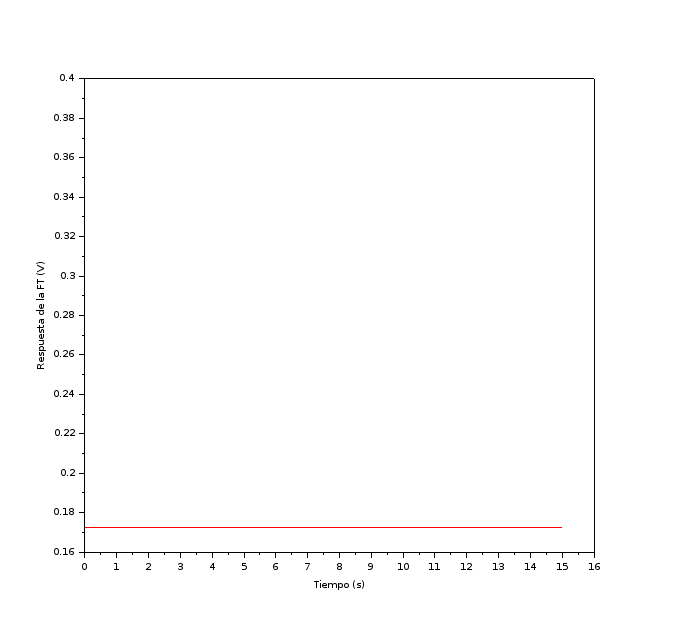
\includegraphics[width=\linewidth]{grafFT}
			\caption{Gráfica función de transferencia en su respuesta temporal con una excitación de escalon unitario.}
			\label{fig:grafFT}
		\end{figure}
		Esta gráfica corresponde al valor de la atenuación de corriente directa:
		\[G_0 = \frac{R_2 \parallel R_3}{R_2 \parallel R_3 + R_1} = 0.1724\]
		\FloatBarrier
		\section{Resultados y discusión}
	\subsection{Simulación con LTspice}
		Se simula el circuito de la figura \ref{cir:hpf} en LTspice, donde se realiza una simulación transitoria para medir las constantes temporales del circuito estudiado. En la figura \ref{fig:circuitos_sim} se muestra el circuito simulado. Se introduce una resistencia en serie para modelar la resistencia en serie de una fuente de voltaje real.
		\begin{figure}[h!]
			\centering
			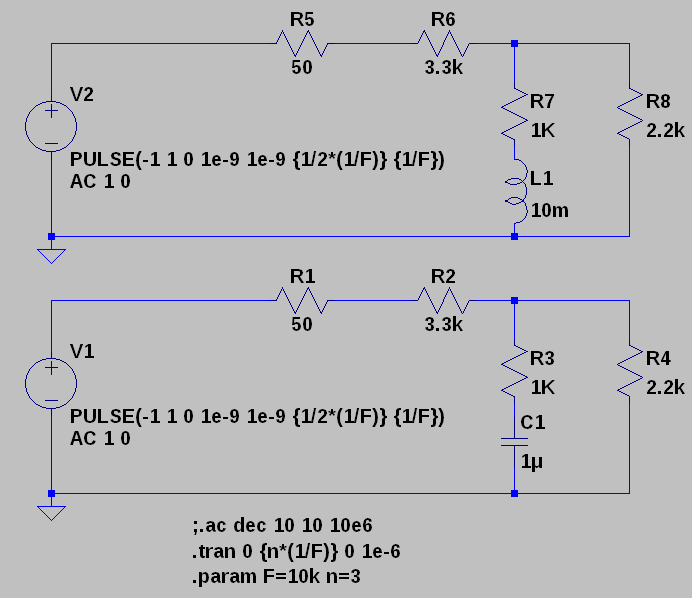
\includegraphics[width=0.7\linewidth]{sim_circuits}
			\caption{Circuitos simulados en LTspice}
			\label{fig:circuitos_sim}
		\end{figure}
		En la figura \ref{fig:circuitos_sim} se estipulan los valores utilizados en la simulación. La medición de las constantes temporales de los circuitos se realiza mediante una fuente de voltaje de onda cuadrada.
		\begin{figure}[h!]
			\centering
			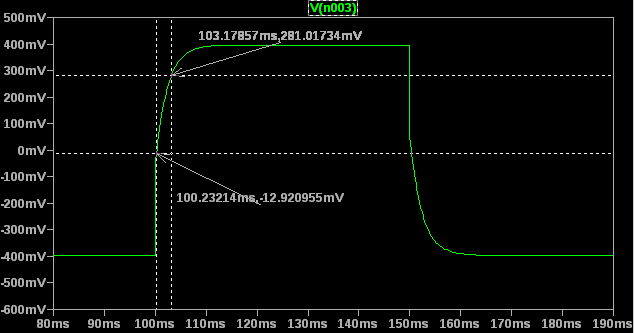
\includegraphics[width=0.7\linewidth]{tau_rc_sim}
			\caption{}
			\label{fig:tau_rc_sim}
		\end{figure}
		\begin{figure}[h!]
			\centering
			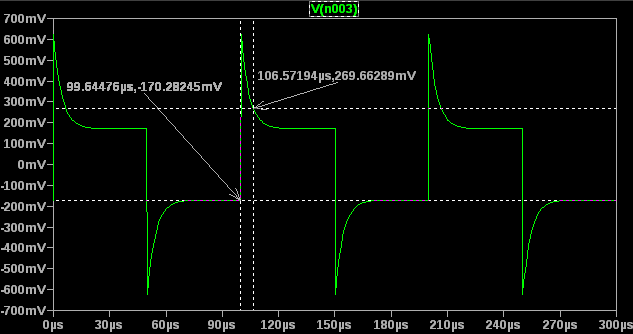
\includegraphics[width=0.7\linewidth]{tau_rl_sim}
			\caption{}
			\label{fig:tau_rl_sim}
		\end{figure}
		Se realizaron las mediciones necesarias y se determina que las constantes de tiempo de los circuitos RL y RC son
		\[ \tau_{RC} = 2.94 \unidad{ms} \]
		\[ \tau_{RL} = 6.92718\unidad{\mu s}\]
		La constante temporal del circuito inductivo se manifiesta en el polo de la función de transferencia con un valor teórico de 
		\[ \tau_{RL} = \frac{10\unidad{mF}}{1\unidad{k \Omega} + 3.35 \unidad{k\Omega} \parallel 2.2 \unidad{k \Omega}} =  4.3 \unidad{\mu s}\]
		Se realiza también el análisis en corriente alterna del circuito con el inductor.
		La salida de esta simulación se muestra en la figura 
		\begin{figure}[h!]
			\centering
			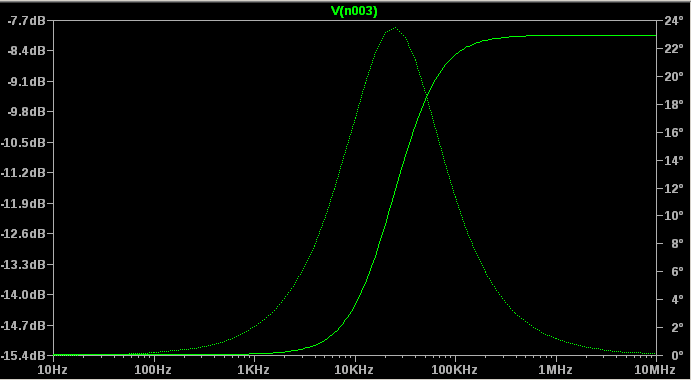
\includegraphics[width=0.7\linewidth]{rl_ac_anal}
			\caption{Respuesta en frecuencia del circuito en la salida.}
			\label{fig:rl_ac_anal}
		\end{figure}
		\FloatBarrier
	\subsection{Mediciones prácticas}
		Se realizan mediciones prácticas para comprobar el comportamiento esperado de la simulación. En las siguientes capturas el osciloscopio se muestran las mediciones de las constantes de tiempo de los circuitos capacitivos e inductivos.
		\begin{figure}[h!]
			\centering
			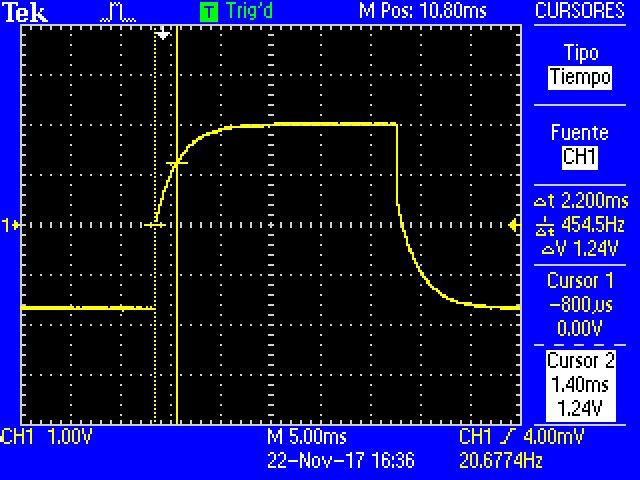
\includegraphics[width=0.7\linewidth]{img/TEK0000}
			\caption{Medición de la constante temporal del circuito capacitivo}
			\label{fig:TEK0000}
		\end{figure}
		\begin{figure}[h!]
			\centering
			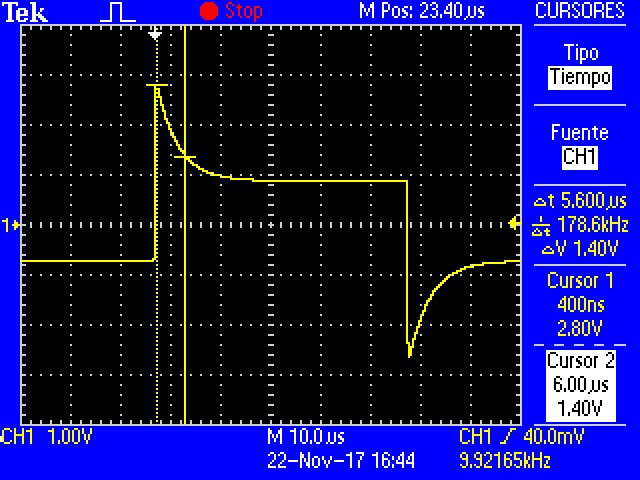
\includegraphics[width=0.7\linewidth]{img/TEK0003}
			\caption{Medición de la constante temporal del circuito inductivo}
			\label{fig:TEK0001}
		\end{figure}		
		\[ \tau_{RC} = 2.2 \unidad{ms} \]
		\[ \tau_{RL} = 5.6\unidad{\mu s}\]
		\FloatBarrier
		Se realiza un barrido de frecuencias desde $10 \unidad{Hz}$ hasta $2 \unidad{MHz}$. La gráfica de las mediciones realizadas se muestra en la figura \ref{fig:med_ac_an}.
		\begin{figure}[h!]
			\centering
			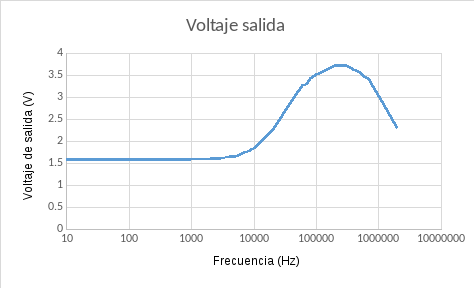
\includegraphics[width=0.7\linewidth]{med_ac_an}
			\caption{Voltaje de salida en respuesta a frecuencia del circuito práctico.}
			\label{fig:med_ac_an}
		\end{figure}
		Se puede observar una considerable desviación en la respuesta en frecuencia del voltaje. Esto se debe a la pobre respuesta del inductor utilizado en la práctica, dado que no es un inductor de alta frecuencia.
	\section{Conclusión}
		En la práctica se revisaron los conceptos analizados en clase, la busqueda e identificación de los ceros y polos de la función de transferencia como una herramienta para identificar la salida del sistema y su respuesta a ciertos estímulos. Estas raíces definen constantes importantes del sistema y tienen a depender fuertemente de todas los factores en el sistema. 

\end{document}